\chapter{A MACHINE LEARNING APPROACH TO QUANTIFYING NOISE IN MEDICAL IMAGES}
\label{chap:automated}

\let\thefootnote\relax\footnotetext{
This chapter previously appeared as:
A. Chowdhury, K.~S. Aggour, S.~M. Gustafson, B. Yener,
``A Machine Learning Approach to Quantifying Noise in Medical Images.''
\emph{Medical Imaging 2016: Digital Pathology},
vol. 9791, pp. 979110U, 2016.}

%%% INTRODUCTION
\section{Introduction}

As advances in medical imaging technology are resulting in significant growth of biomedical image data, new techniques are needed to automate the process of identifying images of low quality. Automation is needed because it is very time consuming for a domain expert such as a medical practitioner or a biologist to manually separate good images from bad ones. While there are plenty of de-noising algorithms in the literature, their focus is on designing filters which are necessary but not sufficient for determining how useful an image is to a domain expert.
Thus a computational tool is needed to assign a score to each image based on its perceived quality. In this paper, we introduce a machine learning-based score and call it the Quality of Image (QoI) score. The QoI score is computed by combining the confidence values of two popular classification techniques support vector machines (SVMs) and Na�ve Bayes classifiers.
We test our technique on clinical image data obtained from cancerous tissue samples. We used 747 tissue samples that are stained by four different markers (abbreviated as CK15, pck26, E\_cad and Vimentin) leading to a total of 2,988 images. The results show that images can be classified as good (high QoI), bad (low QoI) or ugly (intermediate QoI) based on their QoI scores. Our automated labeling is in agreement with the domain experts with a bi-modal classification accuracy of 94 \%, on average. Furthermore, ugly images can be recovered and forwarded for further post-processing.

%%% Data
\section{Data}

The data we use is in the form of microscopic images. The colon cohort in this analysis was collected from the Clearview Cancer Institute of Huntsville Alabama from 1993 until 2002, with 747 patient tumor samples collected as formalin-fixed paraffin-embedded specimens. The median follow-up time of patients in this cohort is 4.1 years, with a maximum of over ten years. Stage 2 patients comprise 38 \% of this cohort, stage 1 and 2 combined are 65 \% of the total patients. We have stained and processed 747 CRC subjects described above on tissue microarrays for 63 target proteins of consequence to cancer biology and ancillary image processing and analysis. A full description of materials and methods was described recently in \cite{gerdes2013highly}.
The images are stained with four different markers. The markers are Ecadherin (E\_cad), pan-Keratin (pck26), Keratin15 (CK15) and Vimentin. The first three markers stain epithelial cells in the tissue, while Vimentin stains mesenchymal cells - a complementary set of cells in the image obtained from the same tissue sample, as shown in Fig. 1. The raw dataset consists of 747 tissue samples and each tissue sample has four images from each marker; resulting in a total of 2,988 images. Since images with the Vimentin marker provides complementary information to the other three markers; we do not use this marker for our analysis and prediction. We do, however, perform preliminary noise reduction on all four markers. The images marked with E\_cad have the least amount of noise associated with them. Images stained with pck26 and CK15 have more noise and undesirable artifacts in them.

\begin{figure}[H]
\centering
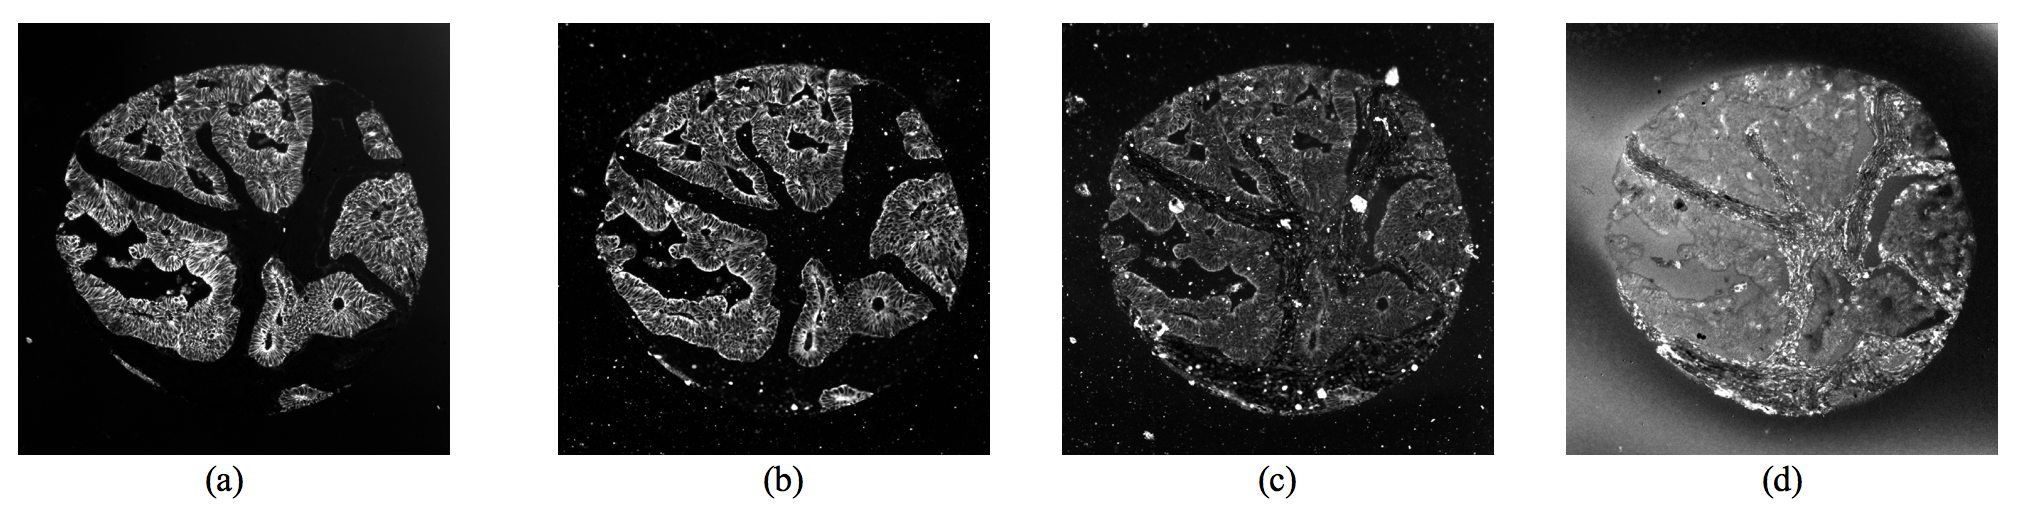
\includegraphics[width=1.0\textwidth]{img/SPIE_example_images}
\caption{Examples of a single colon tumor tissue sample stained with (a) E\_cad (b) pck26 (c) CK15 (d) Vimentin}
\label{fig:SPIE_example_images}
\end{figure}

\subsection{Preliminary noise reduction}
We perform preliminary noise reduction on all four types of images using two techniques. We remove salt and pepper noise using median filtering \cite{huang1979fast} followed by removal of white blob-shaped artifacts using intensity thresholding. Fig. \ref{fig:SPIE_noise_reduction} represents an example of the noise reduction on an image from CK15.  The QoI score (defined in the next section) increases by 67.85 \% on average after noise removal. This shows that the QoI score provides a more accurate estimate after noise removal has been performed. Hence, this step is essential in the process.

\begin{figure}[H]
\centering
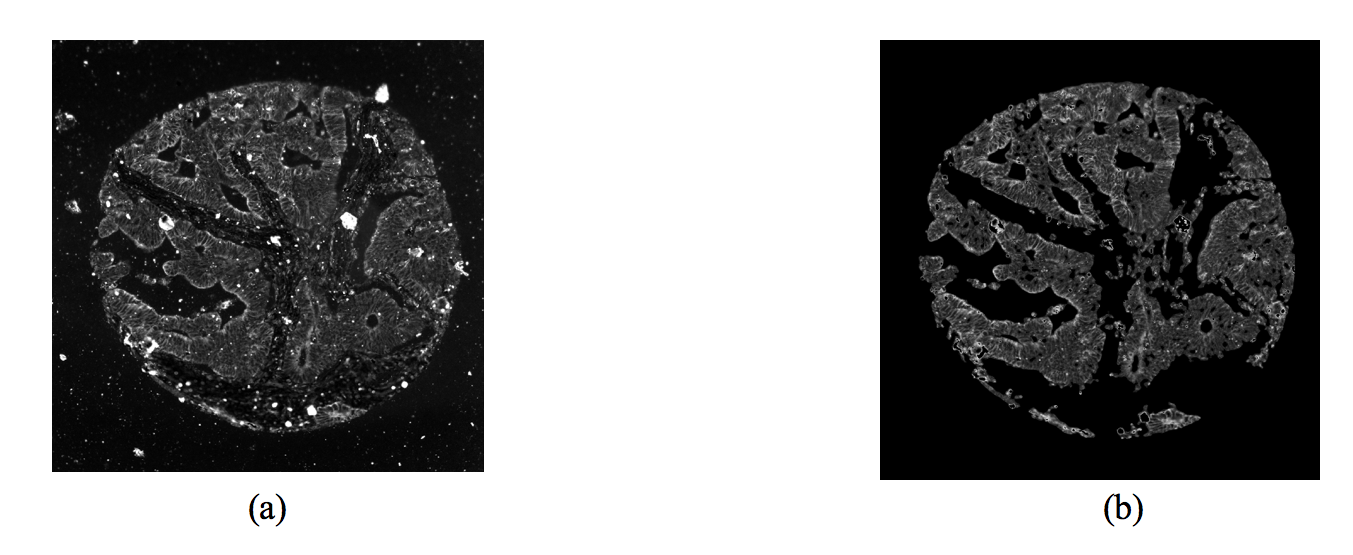
\includegraphics[width=0.9\textwidth]{img/SPIE_noise_reduction}
\caption{ Preliminary noise reduction on an image from CK15 (a) Original image (b) Noise-reduced image
}
\label{fig:SPIE_noise_reduction}
\end{figure}

\subsection{Combination of the three markers}
In addition to the three markers (CK15, pck26, and E\_cad) that we are working with; we use image analysis techniques to form a superimposition of the three markers in such a way that the different types of cells that the markers stain are all present in this one super image. We call this the combined marker. Diffusion like interference exists in the noisy images. The combined image is a way to reduce this kind of noise. The QoI score (defined in the next section) of the combined image is on an average higher (10.76 \%) than the QoI scores of images stained with the rest of the markers for a particular tissue sample. The superposition is performed after preliminary noise elimination. It is done by taking the minimum pixel intensity value among the three images in low intensity regions. We take the maximum intensity value in other regions. An example of this is shown in Fig. \ref{fig:SPIE_combination}. This combination increases the size of the data set; which is inherently imbalanced. It also aids in the recovery of images from the \textit{ugly} class based on the QoI results, as we shall see in the following section.

\begin{figure}[H]
\centering
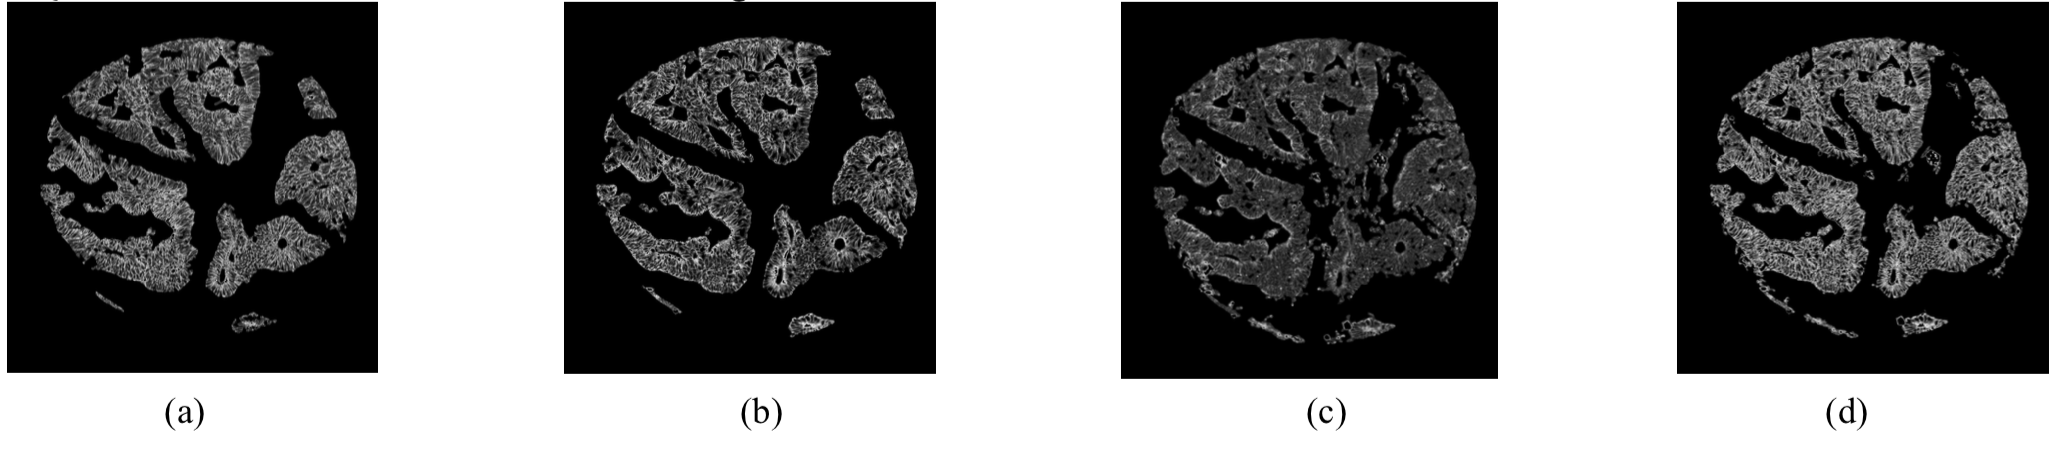
\includegraphics[width=1.0\textwidth]{img/SPIE_combined}
\caption{Images from (a) E\_cad, (b) pck26 and (c) CK15 are used to form the (d) Combined image}
\label{fig:SPIE_combination}
\end{figure}

\subsection{Feature extraction}

We quantify the information in the four markers (E\_cad, pck26, CK15 and Combined) by creating 24 domain-specific features. Features are based on gray-level intensity values, and texture information \cite{haralick1979statistical, haralick1973textural} in the images. 
%The features are shown in Table \ref{table:SPIE_features}.

%\begin{center}
%\begin{longtable}{ | m{6em} | m{10cm} |} 
%\caption{This table represents the various features extracted from the images. Features 9-23 are texture features based on the gray level co-occurence matrix of the image. The sum and difference features (features 14-20) are all measures of homogeneity and texture in the images. The information theoretic features are measures of correlation in the image. We embed a circular mask in the image to mimic the microscopic slide. This is what is meant as circle or circular mask whenever it is used in the formulation of a feature. More information about the features and their respective formulae can be found in \cite{haralick1979statistical, haralick1973textural}.}
% \hline
% Feature & Feature description \\ 
% \hline
% $1$ & Ratio of the size of the objects in the circle to area of the circle \\ 
% \hline
% $2$ & Ratio of the area of objects outside the circular mask to the area outside the circular mask \\  
% \hline
% $3$ & Mean of the gray level pixel values \\ 
% \hline
% $4$ & Second central moment (variance) of the gray level values in the image \\ 
% \hline
%$5$ & Third central moment (skewness) of the gray level values in the image \\ 
% \hline
%$6$ & Fourth central moment (kurtosis) of the gray level values in the image \\ 
% \hline
%$7$ & Energy of the image (quantifies the homogeneity in an image). \\ 
% \hline
%$8$ & Entropy of the image (measures the nonuniformity or complexity of the gray levels in the image) \\ 
% \hline
%$9$ & Texture entropy (measures the nonuniformity or complexity of the texture in the image) \\ 
% \hline
%$10$ & Angular second moment (a measure of homogeneity in the image) \\ 
% \hline
%$11$ & Inverse difference moment (a measure of local homogeneity in an image) \\ 
% \hline
%$12$ & Correlation (represents the linear dependencies of gray levels in the image) \\ 
% \hline
%$13$ & Contrast (a measure of how contrasting the gray level values are in the image) \\ 
% \hline
%$14$ & Sum of squares feature  \\ 
% \hline
%$15$ & Sum variance feature \\ 
% \hline
%$16$ & Sum entropy \\ 
% \hline
%$17$ & Difference average \\ 
% \hline
%$18$ & Difference variance \\ 
% \hline
%$19$ & Difference entropy \\ 
% \hline
%$20$ & Sum average \\ 
% \hline
%$21$ & Information theoretic feature  \\ 
% \hline
%$22$ & Information theoretic feature  \\ 
% \hline
%$23$ & Maximal correlation coefficient \\ 
% \hline
%$24$ & Average intensity of objects in the circle  \\ 
% \hline
% \endlastfoot
% \label{table:SPIE_features}
% \end{longtable}
%\end{center}
In addition to the features, labels are assigned to each image by domain experts based on the amount of noise in them. The label +1 is assigned if the image has some signal in it. This class is colloquially referred to as the \textit{good} class.  Images with a lot of noise in them where there is almost no signal are labelled as -1 or the \textit{bad} class.


\subsection{Data preprocessing}
We use 276x4 (1,104) images as the training set. The four markers (CK15, pck26, E\_cad, and combined) are used corresponding to each tissue sample. The rest of the images (1,884) are used for testing. The test and training sets were selected randomly, with 10-fold cross validation. The data is normalized such that the mean of every feature is 0 and standard deviation is 1.
Singular value decomposition (SVD) is performed to reduce the number of features from 24 such that it captures 95 \% of the information. This reduces the number of dimensions to 12.


\section{Methods and experiments}
In this section, we describe the methods that we used in our analysis of the images and also show the results that we achieved from the application of these methods on our data.

\subsection{Random undersampling}
The data in the two classes is imbalanced because the number of images in the \textit{good} class (images with high amount of signal) far outnumbers the number of instances in the \textit{bad} or noisy class. The ratio of imbalance is approximately 1:30. We perform random undersampling to redress the imbalance and ensure that the sizes of the two classes (good and bad) are the same.

\subsection{Classification and analysis}
We use two popular classification techniques - Support Vector Machines (SVM) and Na�ve Bayes classifiers. The accuracy of the Na�ve Bayes classifier for bi-modal classification on the test set is 96.38 \% and that of SVM is 91.27 \%.

\subsection{Quality of image score}
The models returned by the two classifiers are used to classify the test data as well as assign a score to each test image. The SVM classifier returns a margin value corresponding to each test point. This value is a representation of the distance of the instance from the classifier margin. The margin values are calibrated to fit a probability distribution using \cite{platt1999probabilistic}. The Na�ve Bayes classifier also returns a posterior probability that represents the membership of that point to that class. We combine these two values to form a score that is an indication of the quality of the image. We call this score the \textit{QoI score}. A high QoI score represents a high value of the signal and a small score value indicates that noise predominates the image. 
For image $i$, let $p_{i1}$and $p_{i2}$ be the probabilities returned by SVM and Na�ve Bayes classifiers respectively. Let $l_{i1}$ and $l_{i2}$ be corresponding labels returned the classifier models. The QoI score S is calculated as;

\begin{equation}
\begin{gathered} 
S \ =  \ \sqrt{p_{i1}p_{i2}} \ if \  l_{i1} = l_{i2}\\ 
     = \ 0.5 \ if \  l_{i1}  \neq l_{i2}\\ 
\end{gathered}
\label{eq:1}
\end{equation}

We take the geometric mean of the two scores that we get from each of the two classifiers, if the labelings are in agreement. A score of 0.5 is assigned if they are not. We tested other linear and non-linear functions as well. However, results were mostly invariant for these functions and we observed that the geometric mean was a better representation of the image quality. It is also intuitive that an image should be given the score 0.5 if the two classifiers do not predict the same thing. 
The scores of the test images are normalized such that they vary from 0 to 1; and they form a discrete distribution. The three sample images in Fig.5, (a), (b) and (c) received QoI scores of 0.9995, 0.5001, and 1.7595e-11 respectively using Eq. \ref{eq:1}.


\subsection{Defining the \textit{ugly} class}
In addition to the good and bad class, we observe that there exist some images, which have both quantities of signal and noise in relatively equal proportion. Classifying this kind of image as good or bad becomes very subjective. Therefore, it seems intuitive to define a third class, referred to as the ugly class. We define and extract this class based on the QoI scores in the following manner.
We plot histograms of these discrete distributions as shown in Fig. \ref{fig:ugly_distributions}. We can clearly see from the distributions that the scores form three distinct clusters. Therefore, we performed K-means clustering on the normalized score values with K=3. The cluster of images corresponding to the scores in the middle range is termed the ugly class. Images in the ugly class require further (possibly manual) processing. Thus, we are most interested in the images that are near the middle range, the images that we can recover. 
We threshold out the ugly images with the help of the middle cluster in K-means and using a threshold for scores. The thresholds are taken to be between 0.3 to 0.6. We have found that 7.22 \%, 9.77 \% and 29.30 \% of images in E\_cad, pck26 and CK15 respectively, lie in this middle cluster. The results are intuitive because the amount of noise increases progressively from E\_cad to CK15 to pck26. A number of things may be done with the images that belong to the ugly class. They may be forwarded to medical practitioners for inspection. Further noise elimination may also be performed, or as we have done, the ?combined? image could be used as a proxy for the images belonging to this ugly class. This is because the ?combined? image best captures the important information in the images stained with the three different markers.

 \begin{figure}[H]
\centering
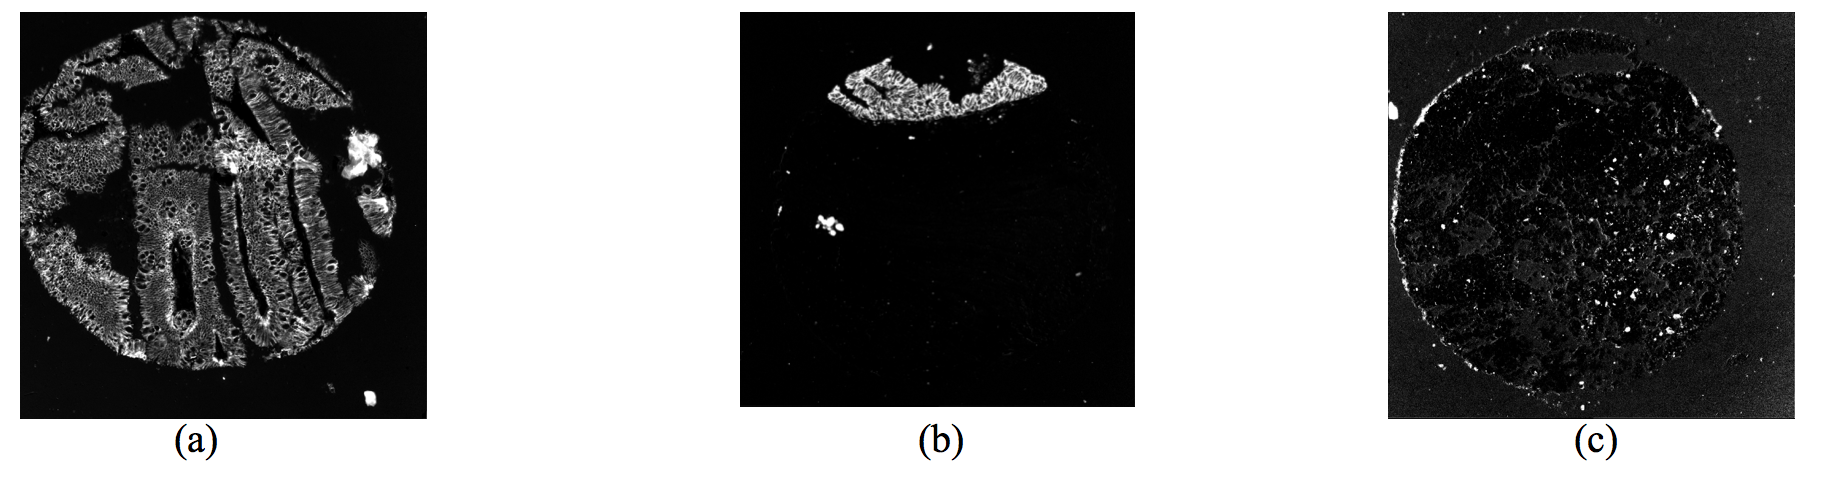
\includegraphics[width=1.0\textwidth]{img/ugly_samples}
\caption{Three sample images from E\_cad stained tissues}
\label{fig:ugly_samples}
\end{figure}

 \begin{figure}[H]
\centering
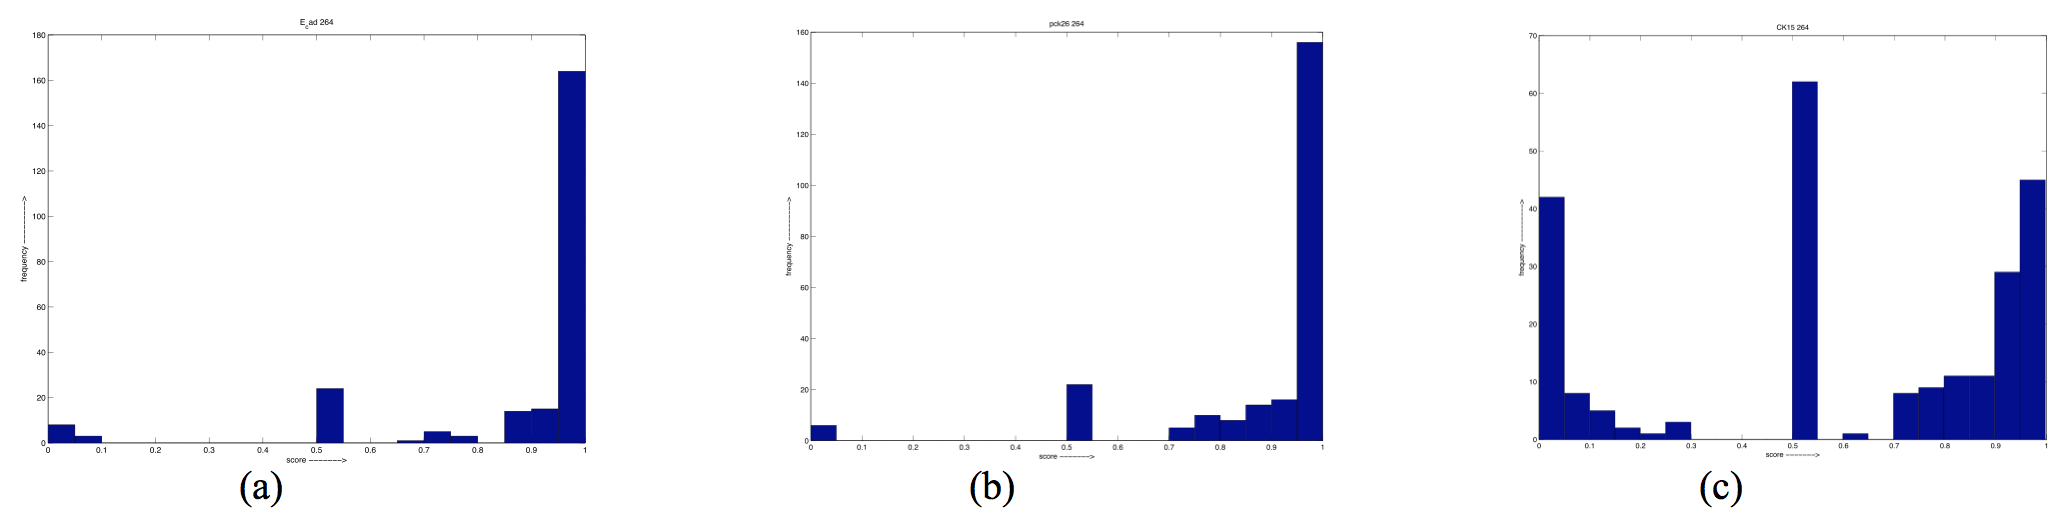
\includegraphics[width=1.0\textwidth]{img/ugly_distributions}
\caption{Discrete distributions of QoI scores for (a) E\_cad (b) pck26 (c) CK15}
\label{fig:ugly_distributions}
\end{figure}

\section{Conclusions}
We introduce in this paper a novel way to combine SVM and Na�ve Bayes classifiers to form an image quality score.  The score is based on the confidence of a data point with respect to the classifier margin; and the distribution of the data captured by the Na�ve Bayes classifier. Images that have high or low information content are easy to label as good or bad respectively. A labeling of the ugly class becomes dependent on the observer. Therefore computing a score is a more natural way of extracting this third class of images. The score helps us retrieve images that may have been discarded by a simple binary classification; or may have gone unnoticed by a human eye. Also, we use image analysis techniques to form a combined image that tries to capture the signal from all three markers.

